\clearpage
\subsection{MSVC: x86 + \olly}

\RU{Попробуем в \olly немного хакнуть программу и сделать вид, что \scanf срабатывает всегда без ошибок.}
\EN{Let's try to hack our program in \olly, forcing it to think \scanf always works without error.}

\RU{Когда в \scanf передается адрес локальной переменной, изначально в этой переменной
находится некий мусор. В данном случае это}\EN{When an address of a local variable is passed into \scanf,
the variable initially contains some random garbage, in this case} \TT{0x6E494714}:

\begin{figure}[H]
\centering
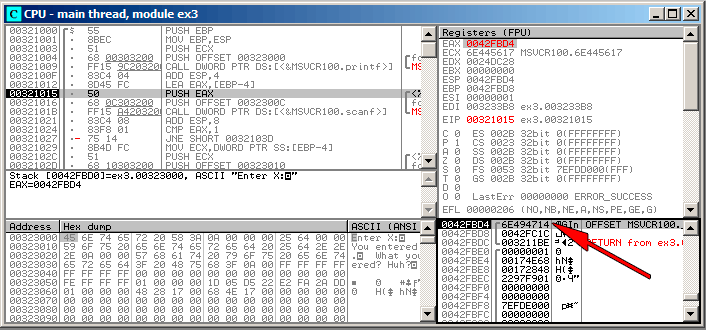
\includegraphics[scale=\FigScale]{patterns/04_scanf/3_checking_retval/olly_1.png}
\caption{\olly: \RU{передача адреса переменной в}\EN{passing variable address into} \scanf}
\label{fig:scanf_ex3_olly_1}
\end{figure}

\clearpage
\RU{Когда}\EN{While} \scanf \RU{запускается, я ввожу в консоли что-то непохожее на число, например}
\EN{executes, in the console I enter something that is definitely not a number, like} \q{asdasd}.
\scanf \RU{заканчивается с 0 в}\EN{finishes with 0 in} \EAX, \RU{что означает, что произошла ошибка}%
\EN{which indicates that an error has occurred}:

\begin{figure}[H]
\centering
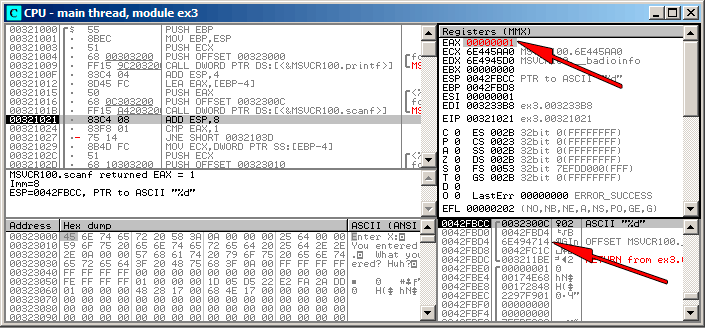
\includegraphics[scale=\FigScale]{patterns/04_scanf/3_checking_retval/olly_2.png}
\caption{\olly: \scanf \RU{закончился с ошибкой}\EN{returning error}}
\label{fig:scanf_ex3_olly_2}
\end{figure}

\RU{Вместе с этим мы можем посмотреть на локальную переменную в стеке~--- она не изменилась.}
\EN{We can also check the local variable in the stack and note that it has not changed.}
\RU{Действительно, ведь что туда записала бы функция \scanf}\EN{Indeed, what would \scanf write there}?
\RU{Она не делала ничего кроме возвращения нуля}\EN{It simply did nothing except returning zero}.

\RU{Попробуем ещё немного \q{хакнуть} нашу программу}\EN{Let's try to \q{hack} our program}.
\RU{Щелкнем правой кнопкой на}\EN{Right-click on} \EAX, \RU{там, в числе опций, будет также}
\EN{Among the options there is} \q{Set to 1}.
\RU{Это нам и нужно}\EN{This is what we need}.

\RU{В \EAX теперь 1, последующая проверка пройдет как надо, и \printf выведет значение переменной
из стека.}
\EN{We now have 1 in \EAX, so the following check is to be executed as intended, 
and \printf will print the value of the variable in the stack.}

\RU{Запускаем (F9) и видим в консоли следующее:}
\EN{When we run the program (F9) we can see the following in the console window:}

\begin{figure}[H]
\centering
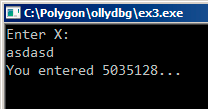
\includegraphics[scale=\FigScale]{patterns/04_scanf/3_checking_retval/olly_3.png}
\caption{\RU{консоль}\EN{console window}}
\end{figure}

\RU{Действительно}\EN{Indeed}, 1850296084 \RU{это десятичное представление числа в стеке}
\EN{is a decimal representation of the number in the stack} (\TT{0x6E494714})!
